%=======================================================================
%  Biomedical Data Processing - final project, retake (August 2026)
%  Written report
%=======================================================================
\documentclass[11pt,a4paper]{article}

\usepackage[utf8]{inputenc}
\usepackage[T1]{fontenc}
\usepackage[margin=2.4cm]{geometry}
\usepackage{amsmath,amssymb}
\usepackage{graphicx}
\usepackage{booktabs}
\usepackage{longtable}
\usepackage{caption}
\usepackage{subcaption}
% Units are handled by these six self-contained macros rather than by siunitx.
% Reason: siunitx v2 provides \SI/\si/\SIrange, siunitx v3 removed them in favour of
% \qty/\unit/\qtyrange, and some installations have neither. Defining them here means this
% file compiles identically on every TeX distribution (MiKTeX, TeX Live, Overleaf) with no
% package-version dependency at all.
\newcommand{\hertz}{Hz}
\newcommand{\second}{s}
\newcommand{\volt}{V}
\newcommand{\decibel}{dB}
\newcommand{\percent}{\%}
\newcommand{\milli}{m}
\newcommand{\micro}{\ensuremath{\mu}}
\newcommand{\num}[1]{#1}
\newcommand{\numrange}[2]{#1--#2}
\newcommand{\si}[1]{#1}
\newcommand{\SI}[2]{#1\,#2}
\newcommand{\SIrange}[3]{#1--#2\,#3}
\usepackage[hidelinks]{hyperref}
\usepackage{xcolor}
\usepackage{titlesec}
\usepackage{enumitem}

\graphicspath{{figures/}}
\setlist{itemsep=2pt,topsep=3pt}
\captionsetup{font=small,labelfont=bf}
\titlespacing*{\section}{0pt}{12pt}{6pt}
\titlespacing*{\subsection}{0pt}{9pt}{4pt}

\newcommand{\change}[1]{\textcolor{black!70}{\textsf{\footnotesize #1}}}
\newcommand{\Q}[1]{\subsection*{#1}}

\title{\vspace{-1.5cm}\textbf{Biomedical Data Processing --- Final Project}\\[2pt]
       \large Retake report: ECG-based identification and EEG-based sleep staging}
\author{Teodora Taleska}
\date{August 2026}

\begin{document}
\maketitle
\vspace{-0.8cm}

\noindent\rule{\textwidth}{0.4pt}
\smallskip

\noindent\textbf{Statement.} This retake was carried out individually. The starting point was
the implementation submitted in the first exam period; every change made since is my own and
is marked in the code with an inline \texttt{\# RETAKE CHANGE} comment. Section~\ref{sec:changes}
lists those changes and maps each one to the section of this report that justifies it.

\smallskip
\noindent\textbf{Deliverables.} \texttt{Part 1/2025\_project\_part1.ipynb} and
\texttt{Part 2/2025\_project\_part2.ipynb}. Both notebooks run top to bottom and write every
figure and table used here into \texttt{report/figures}, so no number in this document is
typed by hand. Part~1 executes in about 30\,s. Part~2 caches its three expensive steps (the
ICA fit, the extracted features and the cross-validation table) in \texttt{Part 2/cache/};
with a cold cache it takes roughly 25 minutes, with a warm cache about 40\,s.

\noindent\rule{\textwidth}{0.4pt}

%=======================================================================
\section{Part I --- ECG-based identification}
%=======================================================================

\subsection{Pipeline}

The recording is a single ECG channel, \SI{605}{\second} at \SI{200}{\hertz}
(\num{121\,006} samples), containing the heartbeats of five subjects in random order. The
identification chain is: R-peak detection with Pan--Tompkins $\rightarrow$ estimation of an
average PQRST template and of a noise-only signal $\rightarrow$ Wiener filtering
$\rightarrow$ re-detection and segmentation into \SI{0.7}{\second} beats $\rightarrow$
\texttt{db4} wavelet decomposition $\rightarrow$ $K$-means with $K=5$, optionally after PCA.
The clustering itself never sees the labels; they are used only to score a finished
partition, through the permutation search in \texttt{match\_labels}.

\subsection{Answers to the overview-sheet questions}

\Q{Which noise sources are present in the ECG?}

Three, all of them stationary, and all three visible in the Welch spectrum of the raw
recording (Fig.~\ref{fig:p1noise}).

\begin{itemize}
  \item \textbf{Baseline wander below \SI{0.7}{\hertz}}, carrying \SI{22.3}{\percent} of the
        total power of the record. Each subject presses on the sensor with a different
        pressure, so the electrode--skin contact potential shifts every time a new person
        touches the electrode.
  \item \textbf{Powerline interference at exactly \SI{50}{\hertz}}, standing \SI{15.1}{\decibel}
        above the local noise floor. There is no line at \SI{60}{\hertz} and no harmonic at
        \SI{100}{\hertz}, which is consistent with a European recording site (the data were
        recorded in Berlin).
  \item \textbf{Broadband muscle and contact noise above roughly \SI{60}{\hertz}}, from small
        finger and forearm contractions while the subject holds the sensor.
\end{itemize}

\change{Change: in the first exam period these three sources were named from the time-domain
trace alone. The question asks \emph{why}, so the answer is now backed by a measurement.}

\begin{figure}[htbp]
  \centering
  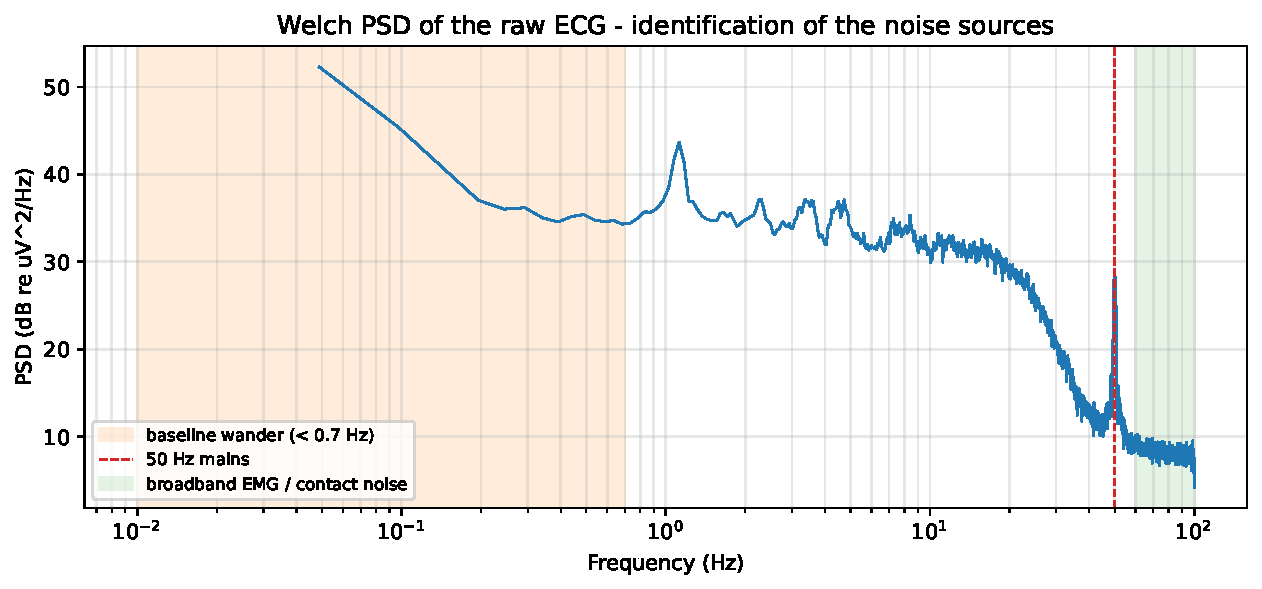
\includegraphics[width=0.78\textwidth]{p1_raw_psd.pdf}
  \caption{Welch PSD of the raw ECG (Hann window, \num{4096} samples,
           \SI{50}{\percent} overlap, $\Delta f = \SI{0.049}{\hertz}$). The resolution is
           deliberately fine so that the narrow mains line can be separated from the
           broadband ECG spectrum.}
  \label{fig:p1noise}
\end{figure}

\Q{How did you compute the Wiener filter? What methods did you use for the PSD estimation?}

The filter is the frequency-domain Wiener solution
\[
  W(f)=\frac{S_d(f)}{S_d(f)+S_n(f)},
\]
built on an $L$-point grid and applied to the full record with weighted overlap-add
(\texttt{wola\_filt}). $S_d$ and $S_n$ are estimated \emph{differently}, because they
describe different kinds of object.

\paragraph{Noise, $S_n$: Welch.} The noise model is the concatenation of all samples that lie
more than \SI{0.4}{\second} after one R-peak and more than \SI{0.3}{\second} before the next.
It is long ($\approx$\,4 minutes) and stationary, so Welch's method is appropriate: Hann
window, \texttt{nperseg}~$=L=512$, \SI{50}{\percent} overlap, \texttt{nfft}~$=L$, two-sided
density scaling. A raw periodogram of a random process has $\approx$\,\SI{100}{\percent}
relative standard deviation regardless of record length; only averaging --- here over about
90 overlapping segments --- makes the estimate usable. The Hann taper suppresses leakage from
the strong low-frequency components into the rest of the band.

\paragraph{Desired signal, $S_d$: periodogram of the zero-padded template.} The averaged
PQRST complex is a single \num{140}-sample \emph{deterministic transient}, not a realisation
of a stationary process. There is nothing to average over, so Welch is the wrong tool. $S_d$
is the periodogram of the mean-removed template zero-padded to $L$, normalised by $f_s N_d$
with $N_d$ the true template length so that its units match those of $S_n$. Zero-padding only
interpolates the frequency axis onto the grid the filter uses; it adds no information and
distorts nothing.

\change{Change: previously $S_d$ was computed with \texttt{welch(nperseg=128, noverlap=64)}
on a \num{140}-sample template. That configuration admits exactly one segment --- the second
would need samples \numrange{64}{191}, which do not exist --- so the call silently returned a
Hann-windowed periodogram of samples \numrange{0}{127} and discarded the last \num{12},
while being described in the overview sheet as an average over overlapping segments.}

\paragraph{Filter length.} $L=512$ (\SI{2.56}{\second}, $\Delta f = \SI{0.391}{\hertz}$),
chosen by the sweep in \S\ref{sec:p1L} rather than assumed. The mean is removed from both the
template and the noise before the PSDs are taken: a DC offset is an artefact of the electrode
contact rather than a feature of the PQRST complex, it would place a large spike at $f=0$ in
$S_d$ and bias the filter towards passing the very baseline wander we are removing, and Wiener
theory assumes a zero-mean noise process.

\begin{figure}[htbp]
  \centering
  \begin{subfigure}{0.49\textwidth}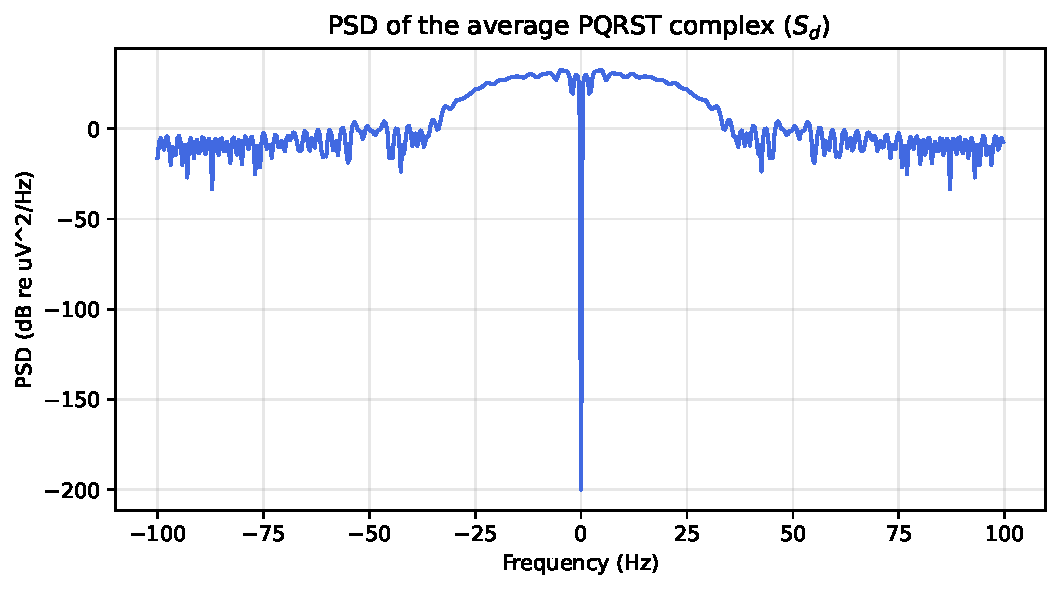
\includegraphics[width=\linewidth]{p1_psd_signal.pdf}\end{subfigure}
  \hfill
  \begin{subfigure}{0.49\textwidth}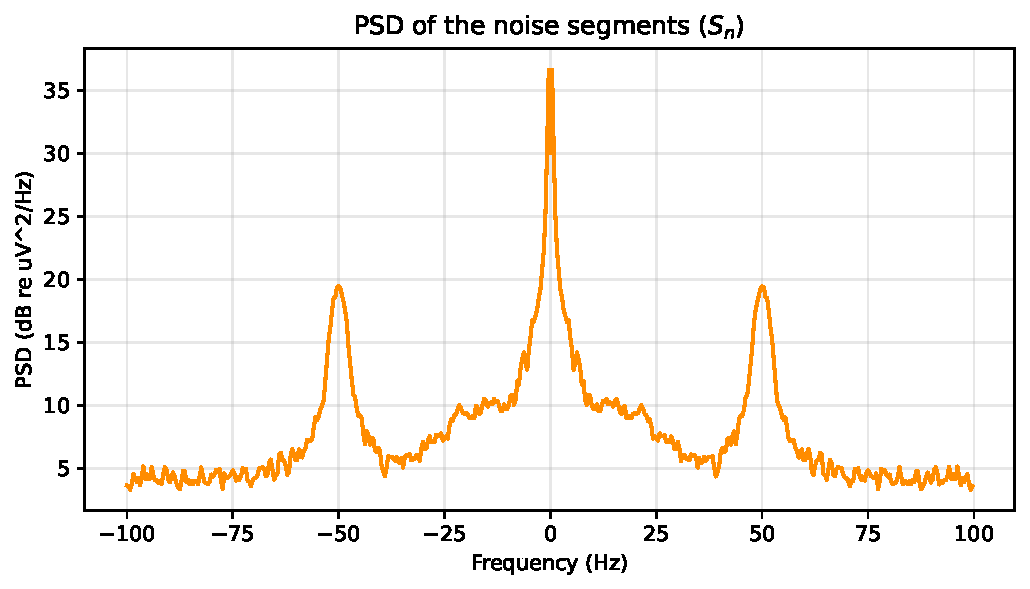
\includegraphics[width=\linewidth]{p1_psd_noise.pdf}\end{subfigure}\\[3pt]
  \begin{subfigure}{0.49\textwidth}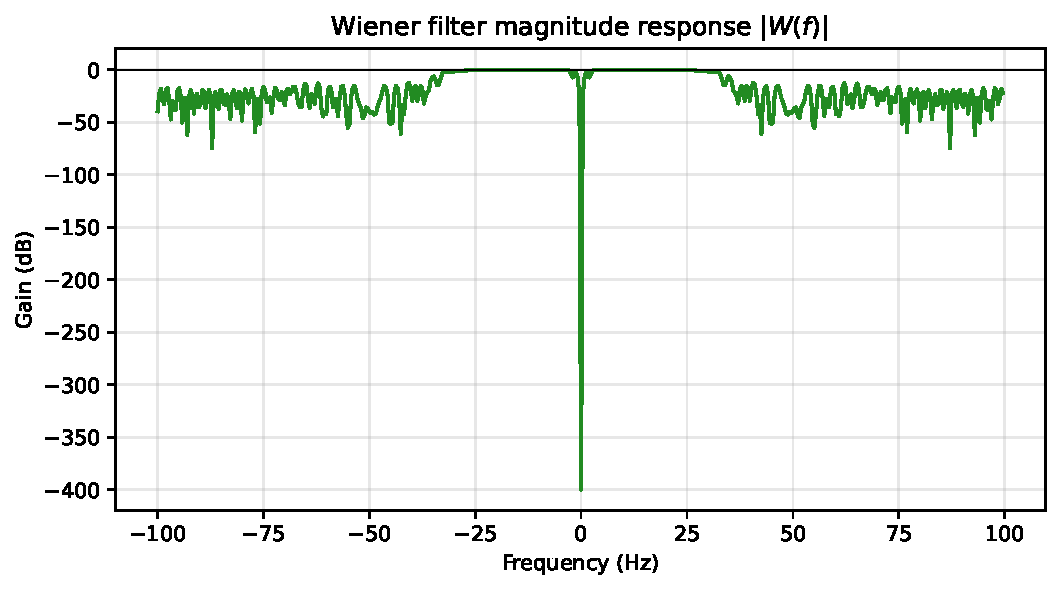
\includegraphics[width=\linewidth]{p1_wiener_tf.pdf}\end{subfigure}
  \hfill
  \begin{subfigure}{0.49\textwidth}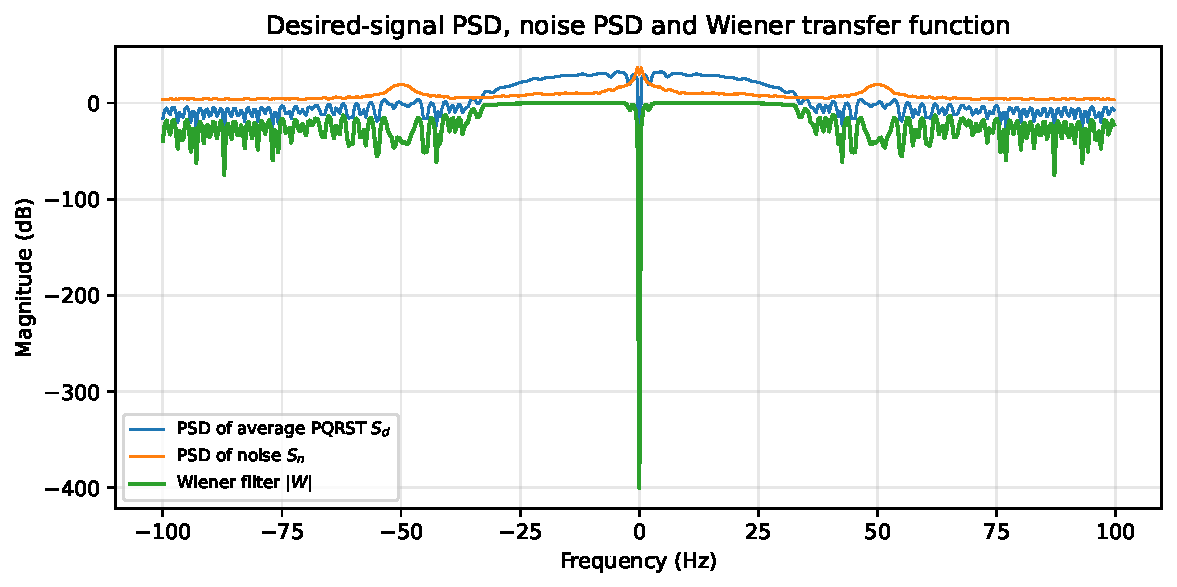
\includegraphics[width=\linewidth]{p1_wiener_overview.pdf}\end{subfigure}
  \caption{Deliverable plots for the Wiener filter. PSDs are plotted as
           $10\log_{10}S$ because a PSD is a power density; the transfer function is plotted
           as $20\log_{10}|W|$ because it is an amplitude gain.
           \change{Change: the two stand-alone PSD plots previously used $20\log_{10}$,
           which doubled their dB axis and contradicted the combined plot.}}
  \label{fig:p1wiener}
\end{figure}

\Q{Did you normalise the wavelet coefficients before classification (without dimensionality
reduction)?}

Yes --- each of the \num{173} coefficients is $z$-scored across segments before $K$-means.
$K$-means minimises a Euclidean criterion, so every dimension contributes to the distance in
proportion to its numerical scale rather than to its information content. The wavelet
sub-bands are on very different scales here: the \texttt{cA5} coefficients track the residual
baseline level and are an order of magnitude larger than the fine-scale \texttt{cD1}
coefficients. Without standardisation the partition is driven by the baseline offset of the
recording session; with it, by the beat morphology. The effect is not marginal:
\textbf{\num{0.489} without standardisation against \num{1.000} with it}
(Table~\ref{tab:p1feat}).

\Q{How did you reduce the feature dimensionality as much as possible? Did you use any
normalisation? If yes, when?}

PCA on the standardised \num{173}-dimensional coefficient matrix, keeping $N=8$ components
(\SI{54.9}{\percent} of the variance). This is a \SI{95}{\percent} reduction in
dimensionality for a loss of \num{0.004} in accuracy ($1.000 \rightarrow 0.9956$).

\emph{Normalisation before PCA: yes.} PCA maximises variance along its components and is
therefore scale-dependent by construction; on unstandardised coefficients PC1 would simply
point along the baseline offset regardless of whether that offset says anything about who the
subject is.

\emph{Normalisation after PCA: no.} The components come out already decorrelated and ordered
by decreasing variance, and that ordering is informative. Re-standardising them would rescale
every component to unit variance and so promote the trailing, mostly-noise directions until
they weigh as much in the $K$-means distance as the leading ones. Measured over ten seeds,
post-PCA scaling is equal or worse at every $N$ tested; at $N=8$ it costs
$0.9956 \rightarrow 0.9882$.

\emph{How $N$ was chosen.} Not by a variance threshold. PCA is unsupervised and maximises
variance, not class separability, so an explained-variance rule is only a proxy for what we
care about --- and here the two disagree sharply: the \SI{90}{\percent} rule would keep
\textbf{\num{40}} components, whereas accuracy has already saturated by $N\approx 8$
(Fig.~\ref{fig:p1pca}). $N=8$ is the elbow of the measured curve.

\begin{table}[htbp]
\centering\small
\caption{Accuracy before and after dimensionality reduction (mean over ten $K$-means seeds).}
\label{tab:p1dr}
\begin{tabular}{lrr}
\toprule
Feature space & Dimensions & Accuracy \\
\midrule
Wavelet coefficients, $z$-scored & 173 & 1.0000 \\
PCA of the same                  &   8 & 0.9956 \\
\bottomrule
\end{tabular}
\end{table}

%-----------------------------------------------------------------------
\subsection{Design choices not covered by the overview sheet}
%-----------------------------------------------------------------------

\subsubsection{Pan--Tompkins parameters, and how the detector was validated}

The detector follows the standard chain: \SI{5}{\hertz}--\SI{11}{\hertz} band-pass (two
4th-order Butterworth sections applied with \texttt{filtfilt}), the five-point derivative
$y[n]=\tfrac{1}{8}(2x[n]+x[n-1]-x[n-3]-2x[n-4])$, squaring, a \SI{150}{\milli\second}
moving-window integrator, peak picking with a minimum inter-beat distance of
\SI{250}{\milli\second} (equivalent to \num{240} beats per minute, comfortably above any
physiological rate), and a $\pm$\SI{100}{\milli\second} local search that moves each detection
onto the true R-peak. Because \texttt{filtfilt} is zero-phase, the band-pass introduces no
group delay to compensate; the derivative is applied causally with \texttt{lfilter}, and the
local search absorbs its delay.

The threshold is a fixed multiple of the mean of the integrated signal rather than the
adaptive dual-threshold scheme with search-back of the original publication. This is a
simplification, and it is defensible here only because the recording is short, the noise is
stationary, and --- as shown next --- it recovers the right number of beats.

\paragraph{Validation.} Each subject only ever measured a single beat at a time, so every run
of constant ground-truth label corresponds to one measurement episode. Dividing each run by
the median run length (\SI{0.94}{\second}) converts the label track into an independent
estimate of the true beat count: \textbf{approximately \num{675} heartbeats}. The detector
finds \num{679} peaks on the raw signal and \num{676} after Wiener filtering, and the
resulting per-subject shares (Table~\ref{tab:p1pct}) match the label track to within half a
percentage point. This estimate is used only to validate the detector and never inside the
algorithm.

\begin{table}[htbp]
\centering\small
\caption{Share of segments per subject, and the independent estimate from the label track.}
\label{tab:p1pct}
\begin{tabular}{lrrrrr}
\toprule
Subject & 1 & 2 & 3 & 4 & 5 \\
\midrule
Segments                    & 117 & 147 & 40 & 115 & 257 \\
Share (\%)                  & 17.31 & 21.75 & 5.92 & 17.01 & 38.02 \\
Estimate from labels (\%)   & 17.4 & 21.3 & 5.9 & 17.3 & 38.1 \\
\bottomrule
\end{tabular}
\end{table}

\subsubsection{Wiener filter length}
\label{sec:p1L}

$L$ sets two things at once: the frequency resolution $\Delta f=f_s/L$ and the length of the
WOLA analysis frame $L/f_s$. It must be at least the \num{140}-sample template length, and
fine enough to separate the narrow \SI{50}{\hertz} line from the ECG band; but a frame
spanning many heartbeats no longer contains a locally homogeneous mixture of signal and noise.

\begin{table}[htbp]
\centering\small
\caption{Effect of the Wiener filter length on the complete pipeline (five $K$-means seeds).
         The true number of heartbeats is approximately \num{675}.}
\label{tab:p1L}
\begin{tabular}{rrrrr}
\toprule
$L$ & Duration (s) & $\Delta f$ (Hz) & Detected beats & Accuracy \\
\midrule
 128 & 0.64  & 1.562 & 844 & 0.4235 \\
 256 & 1.28  & 0.781 & 687 & 0.7910 \\
 \textbf{512} & \textbf{2.56}  & \textbf{0.391} & \textbf{676} & \textbf{1.0000} \\
1024 & 5.12  & 0.195 & 675 & 1.0000 \\
2048 & 10.24 & 0.098 & 672 & 1.0000 \\
\bottomrule
\end{tabular}
\end{table}

The two columns explain each other. At $L=128$ and $L=256$ the resolution is too coarse to
isolate the mains line and the low-frequency roll-off, so the filtered signal still contains
enough noise for Pan--Tompkins to over-detect --- \num{844} and \num{687} peaks against
approximately \num{675} real beats. Those spurious segments are not heartbeats at all, so no
feature representation can cluster them, and a large part of the apparent accuracy loss at
short $L$ is really a segmentation failure. From $L=512$ the beat count is correct and the
accuracy saturates. $L=512$ is the smallest power of two that is both longer than the template
and fine enough in frequency, so it is the value used.
\change{Change: $L=256$ was previously hard-coded with no justification.}

\subsubsection{The desired-signal PSD model, and why the averaged template is the right one}
\label{sec:p1sd}

The assignment asks whether the average PQRST complex should be treated as a template for the
clean signal or for the noisy signal. It is a template for the \textbf{clean} signal: writing
each beat as $x_i[t]=s[t]+n_i[t]$ with zero-mean noise independent from beat to beat,
$\mathbb{E}[\bar x]=s$ and $\operatorname{Var}[\bar x]=\sigma_n^2/N$, so averaging
$N=\num{676}$ aligned beats reduces the noise standard deviation by
$\sqrt{676}\approx 26\times$ before the PSD is taken.

Rather than assert this, the notebook measures it by building a third filter in which $S_d$ is
the average of the periodograms of the \emph{individual, un-averaged} beats --- that is, by
treating the template as a model of signal \emph{plus} noise. Then $S_d\approx S_s+S_n$ and the
filter degenerates to $(S_s+S_n)/(S_s+2S_n)$, which stays within a few decibels of
\SI{0}{\decibel} everywhere and therefore passes the mains line and the baseline wander almost
untouched (Fig.~\ref{fig:p1sd}).

\begin{table}[htbp]
\centering\small
\caption{Identification accuracy for three models of the desired-signal PSD, $L=512$.}
\label{tab:p1sd}
\begin{tabular}{lrr}
\toprule
$S_d$ estimator & Segments & Accuracy \\
\midrule
Periodogram of the averaged template (used)      & 676 & 1.0000 \\
Welch inside the template (first exam period)    & 676 & 1.0000 \\
Average periodogram of the individual noisy beats & 676 & 0.3491 \\
\bottomrule
\end{tabular}
\end{table}

At $L=512$ the estimator used in the first exam period performs identically, because the Hann
taper it applies merely smooths $S_d$ and at this filter length the smoothing is harmless. It
is nevertheless replaced, because it cannot be described correctly: with
\texttt{nperseg}=\num{128} on a \num{140}-sample input it averages a single segment.

\begin{figure}[htbp]
  \centering
  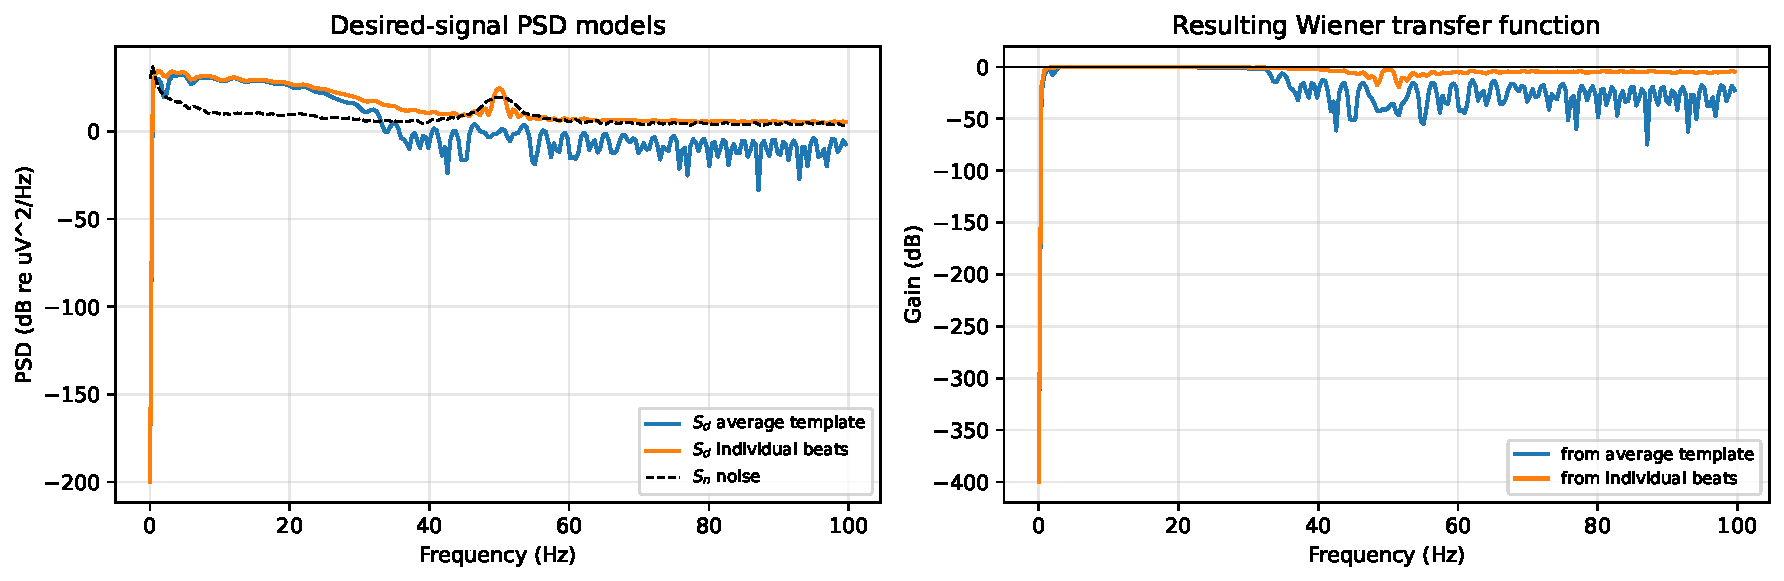
\includegraphics[width=0.92\textwidth]{p1_sd_estimators.pdf}
  \caption{Left: the two candidate models of $S_d$ against the noise PSD. Right: the
           resulting transfer functions. Building $S_d$ from noisy beats yields a filter that
           barely filters.}
  \label{fig:p1sd}
\end{figure}

\subsubsection{The additional Butterworth filter was removed}
\label{sec:p1butter}

The assignment permits an extra Butterworth stage \emph{if the Wiener filtering is deemed
insufficient}. With $L=512$ it is not: the Wiener filter alone recovers the correct number of
beats and perfect clustering. The \SI{5}{\hertz}--\SI{40}{\hertz} band-pass used in the first
exam period is also questionable in principle, since a \SI{5}{\hertz} high-pass removes most
of the P-wave, the T-wave and the ST segment --- exactly the morphological detail that
distinguishes one subject from another.

\begin{center}\small
\begin{tabular}{lrr}
\toprule
Extra Butterworth & Segments & Accuracy \\
\midrule
none (used) & 676 & 1.0000 \\
\SIrange{0.5}{40}{\hertz} & 676 & 0.9964 \\
\SIrange{1}{40}{\hertz} & 676 & 1.0000 \\
\SIrange{5}{40}{\hertz} (first exam period) & 676 & 0.9985 \\
\bottomrule
\end{tabular}
\end{center}

Consequently the pipeline segments the Wiener output directly and the third deliverable plot
(a Butterworth-filtered window with annotated R-peaks) is not required. Edge effects were
checked instead: WOLA weights both analysis and synthesis with $\sqrt{\text{Hann}}$ and hops
by half a frame, so the squared windows sum to a constant and reconstruction is exact in the
interior. The only genuine artefact is the final incomplete frame --- \num{174} samples,
\SI{0.87}{\second}, \SI{0.14}{\percent} of the record --- which is removed by the boundary
condition in the segmentation step.

\subsubsection{Feature representation: coefficients, not sub-band energies}
\label{sec:p1feat}

This is the single largest change in Part~I. \texttt{pywt.wavedec(seg, 'db4', level=5)}
returns $[\texttt{cA5},\texttt{cD5},\texttt{cD4},\texttt{cD3},\texttt{cD2},\texttt{cD1}]$;
concatenated, that is \textbf{\num{173} coefficients} per \num{140}-sample segment, with the
sub-bands covering the octaves \SIrange{0}{3.1}{\hertz} (\texttt{cA5}, P-wave and baseline)
up to \SIrange{50}{100}{\hertz} (\texttt{cD1}). Each coefficient is an inner product of the
segment with a wavelet at a given scale \emph{and position}, so the representation encodes
how much activity of a given band occurs at a given moment in the beat.

In the first exam period each segment was reduced instead to the \emph{energy} of each
sub-band --- $\sum \texttt{cD3}^2$ and $\sum \texttt{cD4}^2$ for the clustering, six energies
for the PCA. Summing squares within a band discards where in the beat the energy occurs and
collapses \num{173} numbers into six; what remains is essentially a six-bin power spectrum, so
two subjects whose QRS complexes carry equal energy but differ in shape or timing become
indistinguishable. It also left the dimensionality-reduction section with almost nothing to
reduce.

\begin{table}[htbp]
\centering\small
\caption{Effect of the feature representation, mean $\pm$ std over ten $K$-means seeds.}
\label{tab:p1feat}
\begin{tabular}{lrr}
\toprule
Representation & Dimensions & Accuracy \\
\midrule
6 sub-band energies, $z$-scored \change{(first exam period)} & 6 & $0.7219 \pm 0.0000$ \\
6 sub-band energies, raw                                     & 6 & $0.3609 \pm 0.0000$ \\
173 wavelet coefficients, raw                                & 173 & $0.4886 \pm 0.0018$ \\
\textbf{173 wavelet coefficients, $z$-scored (used)}         & \textbf{173} & $\mathbf{1.0000 \pm 0.0000}$ \\
\bottomrule
\end{tabular}
\end{table}

\paragraph{Decomposition level.} With \num{140} samples and \texttt{db4} (filter length 8) the
deepest level free of boundary effects is $\lfloor\log_2(140/7)\rfloor = 4$, so PyWavelets
warns at level~5. The level is prescribed by the assignment and is kept. The default
\texttt{symmetric} extension applies the same boundary treatment to every segment, so the
distortion is common to all of them and does not affect the \emph{relative} comparison that
the clustering is based on.

\paragraph{Which two coefficients are plotted.} The identification algorithm may not use the
labels, so the two display coefficients are selected by an unsupervised criterion: the
coefficient with the largest absolute loading on PC1 and the one with the largest absolute
loading on PC2 of the standardised coefficient matrix. These are the two individual features
carrying most of the between-segment variation, and they are near-independent, which is what
makes them useful as the axes of a scatter plot. The criterion selects
\texttt{cD3[9]} and \texttt{cD4[14]} --- both inside the \SIrange{6}{25}{\hertz} octaves, i.e.
the QRS complex, which is physiologically the most subject-specific part of the beat. The
obvious alternative, largest raw variance, selects \texttt{cA5} coefficients, which track the
residual baseline level and separate recording sessions rather than morphology.

\subsubsection{$K$-means settings and run-to-run stability}

$K=5$ is given by the problem. \texttt{n\_init=10} and \texttt{random\_state=42} are fixed so
the notebook is reproducible. Lloyd's algorithm converges to a \emph{local} minimum whose
identity depends on the random initialisation, so the assignment's question about
reproducibility is answered by measurement rather than assertion: over ten seeds the standard
deviation of the accuracy is exactly \num{0} in the full coefficient space and for every
$N\ge 6$ after PCA, because the five subjects form well-separated compact groups there.
Visible seed-to-seed variation appears only in the strongly compressed representations
($N=2$: $0.8466 \pm 0.0019$), which is the situation the question points at.

Cluster \emph{labels} are arbitrary --- any permutation of the five indices describes the same
partition --- so accuracy is only meaningful after the best of the $5!=120$ permutations has
been applied, which is what \texttt{match\_labels} does.

\begin{figure}[htbp]
  \centering
  \begin{subfigure}{0.48\textwidth}
    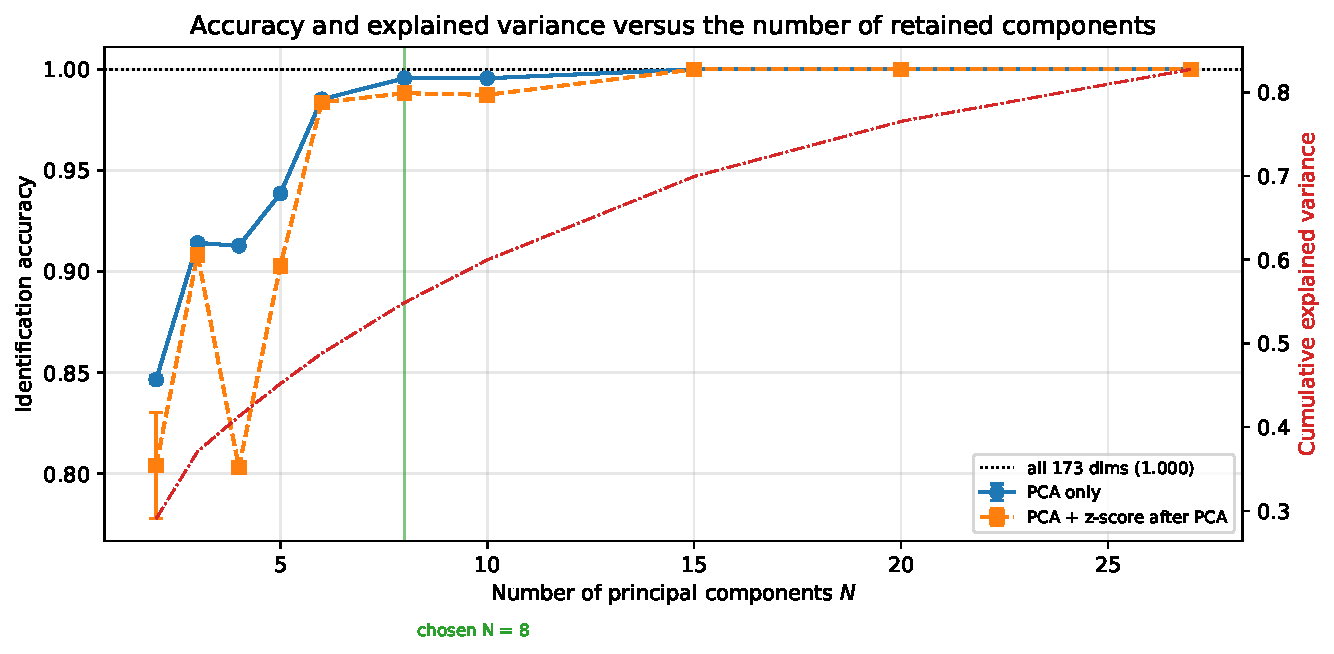
\includegraphics[width=\linewidth]{p1_sweep_pca.pdf}
    \caption{Accuracy and cumulative explained variance versus $N$.}
    \label{fig:p1pca}
  \end{subfigure}\hfill
  \begin{subfigure}{0.48\textwidth}
    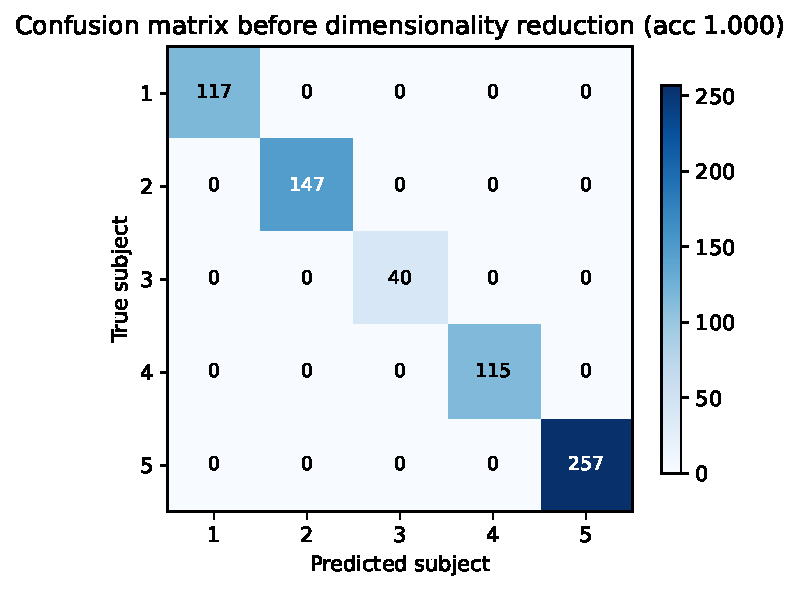
\includegraphics[width=\linewidth]{p1_cm_before_dr.pdf}
    \caption{Confusion matrix, 173-D coefficients.}
  \end{subfigure}
  \caption{Dimensionality reduction. The accuracy curve saturates around $N=8$, at which point
           only \SI{55}{\percent} of the variance is retained --- the \SI{90}{\percent} rule
           would keep \num{40} components.}
\end{figure}

\subsection{Results}

Clustering the \num{676} segments in the standardised \num{173}-dimensional wavelet space
recovers the five subjects \textbf{exactly} (accuracy \num{1.000}; the confusion matrix is
diagonal, with 117, 147, 40, 115 and 257 segments correctly assigned). After PCA to eight
dimensions the accuracy is \num{0.9956}, with three segments of subject~1 assigned to
subject~2.

\paragraph{A caveat on the perfect score.} This is a small, controlled problem: five subjects,
one sensor, one recording session each, and one of the five (subject~3) has valvular disease,
which makes their beats morphologically unmistakable. It should not be read as evidence that
ECG biometrics generalise at this level --- with more subjects, recordings on different days,
or different electrode positions, within-subject variability would grow and the between-subject
margins would shrink. Note also that subject~3 contributes only \SI{5.9}{\percent} of the
segments, so a degenerate clustering that merged that subject into a neighbour would still
score \SI{94}{\percent}; this is why the confusion matrix, and not only the scalar accuracy,
is reported.

%=======================================================================
\section{Part II --- EEG-based sleep staging}
%=======================================================================

\subsection{Pipeline}

Twenty overnight PSG recordings, four channels (Fpz-Cz, Pz-Oz, EOG, EMG) at \SI{100}{\hertz},
segmented into \SI{30}{\second} epochs: \num{21\,357} epochs in total, \num{15\,760} from the
training subjects \numrange{0}{14} and \num{5597} from the held-out subjects
\numrange{15}{19}. The chain is: FastICA artefact removal, \SIrange{0.5}{30}{\hertz}
band-pass, Welch PSD and band-power features, leave-one-subject-out model selection, and
finally retraining on all training subjects with a single evaluation on the held-out subjects.

\subsection{Answers to the overview-sheet questions}

\Q{What visible patterns characterise each sleep stage?}

The five epochs discussed below all come from subject~6; epoch indices are given for each.

\begin{itemize}
  \item \textbf{Wake (epoch 5).} Fast, irregular, relatively high-amplitude EEG. Physiologically
        wakefulness shows low-amplitude beta, with alpha (\SIrange{8}{12}{\hertz}) when the
        eyes are closed and the subject is relaxed; much of the visible amplitude here is in
        fact ocular and muscular contamination, which is what the ICA step removes. The
        supporting evidence is in the reference channels: frequent large EOG deflections and
        the \emph{highest} EMG level of the five epochs, reflecting active postural muscle tone.
  \item \textbf{N1 (epoch 64).} The EEG slows and its amplitude falls; alpha drops out and theta
        (\SIrange{4}{8}{\hertz}) dominates. N1 has no positive defining marker --- it is
        recognised by the \emph{absence} of both alpha and the N2 markers --- which is what makes
        it the hardest stage to score. The EOG shows slow rolling deflections rather than the
        sharp movements of wake.
  \item \textbf{N2 (epoch 74).} Medium-amplitude theta background interrupted by
        \textbf{sleep spindles}: \SIrange{11}{16}{\hertz} bursts lasting about a second, one
        visible near $t=\SI{25}{\second}$. K-complexes (a sharp negative deflection followed by
        a positive component) may also occur. The EOG is quiet and the EMG is further reduced.
  \item \textbf{N3 (epoch 173).} Large-amplitude, slow, strongly synchronised delta activity
        below \SI{4}{\hertz}; the trace is markedly more regular than in the lighter stages.
        Ocular contamination is still visible in the EEG channels even here, which is why
        artefact removal precedes every feature computation.
  \item \textbf{REM (epoch 255).} A low-amplitude, mixed-frequency EEG that resembles wake ---
        hence ``paradoxical'' sleep --- but the reference channels resolve the ambiguity:
        distinct \emph{rapid} EOG deflections, and the \emph{lowest} EMG level of all five
        epochs, reflecting REM muscle atonia.
\end{itemize}

The last point drives a modelling decision. Wake and REM are nearly indistinguishable on the
EEG channel alone and are separated almost entirely by the EOG and EMG channels, which is why
those channels are evaluated as \emph{features} in Task~4 and not only as artefact references.

\Q{What is the effect of including versus excluding EOG/EMG channels from ICA input?}

Including them is what makes the problem solvable, for two distinct reasons.

\begin{enumerate}
  \item \textbf{Identifiability.} ICA can separate at most as many sources as it has input
        channels. With four inputs it resolves four sources; with the two EEG derivations alone
        it could resolve two, fewer than the number of physically present sources (cortical
        activity on two derivations, ocular, muscular). The ocular and muscular contributions
        would then necessarily remain mixed into the EEG components.
  \item \textbf{Labelling.} Even if a two-channel ICA did isolate an artefact, nothing would
        say \emph{which} component it is. The automatic rule needs a reference signal to
        correlate against, and the EOG and EMG channels are exactly that. This is not merely
        convenient here: as \S\ref{sec:p2emg} shows, the components cannot be told apart by
        their spectra in this dataset, so the reference channels are necessary.
\end{enumerate}

The cost is that two of four components are discarded, so the reconstruction is rank-deficient
and whatever genuine cortical activity projected onto them is lost with the artefacts. That is
the standard trade-off of ICA-based artefact rejection, and it is one reason the EOG and EMG
channels are re-introduced as separate features rather than discarded entirely.

\Q{Should filtering be done before or after ICA artefact removal? Why?}

\textbf{After} --- ICA first, band-pass second, which is the order used.

ICA models each observation as an \emph{instantaneous linear mixture} $x[t]=A\,s[t]$ and
estimates a single mixing matrix $A$ from the joint amplitude distribution of the four
channels. Filtering first breaks that model: a band-pass is applied per channel and affects the
underlying sources differently depending on where their energy lies, so the observed data are
no longer an instantaneous mixture with one constant matrix. Filtering first would also remove
the evidence the identification step needs --- the artefacts are characterised precisely by the
frequency ranges a \SIrange{0.5}{30}{\hertz} band-pass attenuates, so the correlations against
the reference channels would weaken. The reverse argument does not apply: nothing about the
band-pass depends on the artefacts having been removed, so there is no cost to placing it
second.

A caveat worth stating: a very large drift can degrade the ICA estimate itself, and the usual
remedy is a gentle high-pass well below the band of interest \emph{before} ICA with the full
band-pass afterwards. That was not needed here --- the components separate cleanly, with
$|r|>0.997$ against the reference channels for all twenty subjects.

\Q{Describe the pipeline that worked best, including preprocessing, model and hyperparameters.
Why is this the best model?}

\begin{center}\small
\begin{tabular}{ll}
\toprule
Features & Welch PSD of Fpz-Cz, \SIrange{0.5}{30}{\hertz}, \SI{3}{\second} segments, in dB (89 bins) \\
         & plus 5 EOG/EMG features (94 in total) \\
Normalisation & $z$-score within each recording, then a global \texttt{StandardScaler} \\
Model    & \texttt{SVC}, RBF kernel \\
Hyperparameters & $C=1.0$, \texttt{gamma='scale'}, \texttt{class\_weight='balanced'} \\
\midrule
LOSO accuracy    & $0.780 \pm 0.098$ \\
LOSO F1-macro    & $\mathbf{0.727 \pm 0.101}$ \\
LOSO F1-weighted & $0.794 \pm 0.091$ \\
\bottomrule
\end{tabular}
\end{center}

Three observations drive the choice.

\textbf{The preprocessing matters more than the classifier.} Averaged over classifier families,
F1-macro ranges from \num{0.598} to \num{0.702} across the seven preprocessing configurations,
whereas within the plain PSD block the nine classifier settings span only \num{0.578} to
\num{0.671} (Table~\ref{tab:p2prep}). The largest single gain is per-recording normalisation.
The reason is physical rather than statistical: absolute EEG amplitude depends on skull
thickness, electrode impedance, age and amplifier gain, so different nights sit at different
absolute dB levels, and those offsets are larger than the between-stage differences the
classifier must detect. A global \texttt{StandardScaler} cannot remove them because it
subtracts the \emph{grand} mean over all training epochs, not each recording's own offset.
Normalising within a recording turns the features into ``deviation from this person's average
night''.

\textbf{The EOG/EMG features fix the stages the EEG cannot separate.} Adding five features
derived from the reference channels raises the best F1-macro from \num{0.675} to \num{0.727}.
Wake and REM have similar EEG spectra; the EMG envelope separates them almost by itself
(Cohen's $d = 7.10$ between Wake and REM on subject~6).

\textbf{Among classifiers, the RBF SVM is strongest.} With \num{94} standardised features and
about \num{15000} training epochs, an RBF kernel can represent the curved boundaries between
neighbouring stages, and the margin formulation is comparatively robust in a moderately
high-dimensional space where $k$-NN distances become uninformative and single trees find
unstable splits. Logistic regression is close behind (\num{0.722}), which suggests the classes
are close to linearly separable once the features are right --- another sign that the
representation, not the model, is doing the work. \texttt{class\_weight='balanced'} trades
about two points of accuracy for a larger gain in F1-macro, which is the intended trade given
the selection criterion (on the plain PSD block: $0.654 \rightarrow 0.671$ F1-macro while
accuracy falls $0.783 \rightarrow 0.755$).

\begin{table}[htbp]
\centering\small
\caption{Mean and best F1-macro per preprocessing configuration across the classifier families.}
\label{tab:p2prep}
\begin{tabular}{lrrr}
\toprule
Preprocessing & Features & Mean F1-macro & Best F1-macro \\
\midrule
PSD plus EOG/EMG, per-recording $z$-score \textbf{(used)} & 94 & \textbf{0.702} & \textbf{0.727} \\
PSD, per-recording $z$-score                             & 89 & 0.650 & 0.675 \\
PSD, global scaling only                                 & 89 & 0.632 & 0.671 \\
PSD then PCA, 10 components                              & 10 & 0.629 & 0.672 \\
$\log_{10}$ band power, 2 channels                       & 10 & 0.623 & 0.655 \\
Relative band power, 2 channels                          & 10 & 0.616 & 0.641 \\
dB PSD averaged in the 5 bands, 2 channels               & 10 & 0.598 & 0.650 \\
\bottomrule
\end{tabular}
\end{table}

\Q{How does the model perform on the held-out test set, and how does that compare to the
cross-validation performance?}

On subjects \numrange{15}{19} (\num{5597} unseen epochs) the deployed pipeline reaches
\textbf{accuracy \num{0.780}}, \textbf{F1-macro \num{0.719}} and F1-weighted \num{0.794}.

\begin{table}[htbp]
\centering\small
\caption{Classification report on the held-out subjects, with the first exam period for
         comparison.}
\label{tab:p2report}
\begin{tabular}{lrrrrr}
\toprule
Stage & Precision & Recall & F1 & Support & F1, first exam period \\
\midrule
Wake & 0.749 & 0.760 & 0.754 & 890  & 0.728 \\
N1   & 0.269 & 0.621 & 0.375 & 264  & 0.062 \\
N2   & 0.891 & 0.792 & 0.838 & 2351 & 0.817 \\
N3   & 0.813 & 0.827 & 0.820 & 958  & 0.800 \\
REM  & 0.853 & 0.768 & 0.808 & 1134 & 0.641 \\
\midrule
Accuracy    & \multicolumn{3}{c}{0.780} & 5597 & 0.744 \\
Macro avg   & 0.715 & 0.753 & 0.719 & 5597 & 0.610 \\
Weighted avg& 0.818 & 0.780 & 0.794 & 5597 & 0.729 \\
\bottomrule
\end{tabular}
\end{table}

The test result is very close to the cross-validated estimate --- F1-macro \num{0.719} against
\num{0.727}, accuracy \num{0.780} against \num{0.780} --- which is the useful outcome: the LOSO
protocol, computed only on subjects \numrange{0}{14}, predicted performance on five subjects the
model had never seen. The small drop is what one expects when moving from a validation estimate
to a single held-out evaluation, and it does not indicate overfitting.

The pooled number should be read alongside the per-subject breakdown, because the spread across
nights is much wider than the gap between the CV and test means:

\begin{center}\small
\begin{tabular}{lrrrrr}
\toprule
Subject & 15 & 16 & 17 & 18 & 19 \\
\midrule
Epochs   & 952 & 1144 & 1002 & 964 & 1535 \\
Accuracy & 0.871 & 0.742 & 0.734 & 0.771 & 0.787 \\
F1-macro & 0.814 & 0.690 & 0.629 & 0.716 & 0.722 \\
\bottomrule
\end{tabular}
\end{center}

Performance depends more on \emph{which} subject is being scored than on the train/test split,
which is also why the LOSO fold standard deviation ($\pm 0.101$ on F1-macro) is large.

\begin{figure}[htbp]
  \centering
  \begin{subfigure}{0.42\textwidth}
    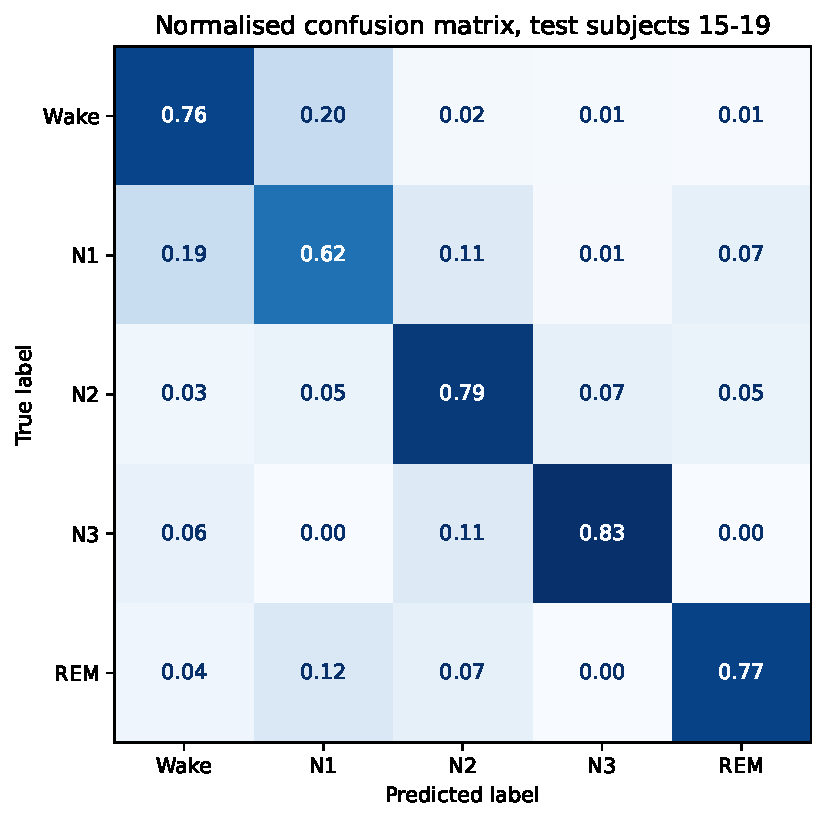
\includegraphics[width=\linewidth]{p2_confusion_test.pdf}
    \caption{Normalised confusion matrix, subjects 15--19.}
  \end{subfigure}\hfill
  \begin{subfigure}{0.55\textwidth}
    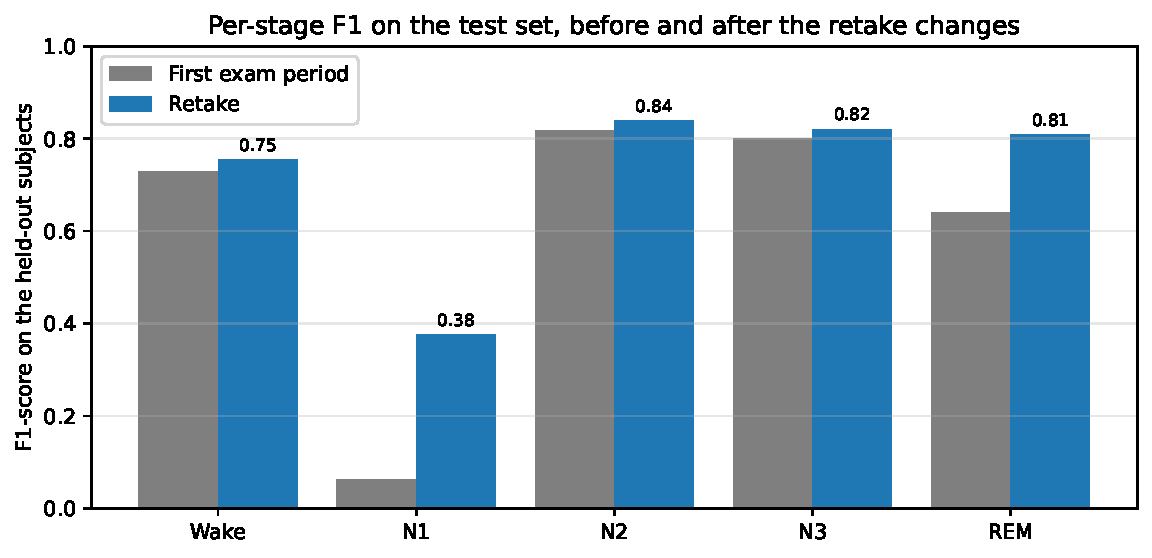
\includegraphics[width=\linewidth]{p2_per_class_f1.pdf}
    \caption{Per-stage F1 before and after the retake changes.}
  \end{subfigure}
  \caption{Test-set performance. Every stage improved; N1 rose from F1 \num{0.062} to
           \num{0.375} and REM from \num{0.641} to \num{0.808}.}
\end{figure}

%-----------------------------------------------------------------------
\subsection{Design choices not covered by the overview sheet}
%-----------------------------------------------------------------------

\subsubsection{ICA: fitting data, reshaping, and how much data is needed}
\label{sec:p2ica}

\texttt{FastICA.fit} expects \texttt{(n\_samples, n\_features)}, where a feature is a recording
channel and a sample is one instant in time. The raw array is
\texttt{(n\_epochs, n\_channels, n\_samples)}, so time and channels are swapped and the first
two axes are collapsed, giving \texttt{(n\_epochs $\times$ n\_samples, 4)}. Collapsing epochs is
legitimate because ICA has no notion of time order --- it models each observation as an
instantaneous mixture --- so the discontinuities at epoch boundaries are irrelevant.

The model is fitted on the \textbf{training subjects only} (\numrange{0}{14}) and then applied
unchanged to the test subjects, so no information from subjects \numrange{15}{19} enters the
preprocessing. \texttt{random\_state} is fixed, because FastICA starts from a random unmixing
matrix and neither the sign nor the order of the recovered components is identified by the
model.

\change{Change: the fit now uses a seeded random subsample of \num{100\,000} samples per subject
(\num{1\,500\,000} by 4) instead of all \num{47\,280\,000} by 4 samples. The quantity being estimated is
a single $4\times4$ unmixing matrix --- sixteen parameters --- and FastICA converges long before
millions of samples; the full fit cost minutes and bought nothing. The notebook verifies the
claim by re-estimating on a four times larger disjoint subsample and comparing the mixing
directions after removing the sign and permutation ambiguity: the best cosine similarities are
$[1.000, 0.9999, 1.000, 1.000]$.}

\subsubsection{Automatic component selection}
\label{sec:p2sel}

Each component's concatenated time series is correlated with the EOG and EMG reference channels
of the same subject, and the component with maximum $|r|$ against each reference is zeroed
before the inverse transform. The selection is recomputed per subject, so the procedure adapts
to per-recording differences in the mixing.

\change{Change: the selection is now audited. The notebook prints, for all twenty subjects,
which component was chosen and how strong the association was, and flags the case where the
same component would be nominated for both references (it never occurs).} The correlations are
extremely high --- $|r| \ge 0.998$ for every subject --- and the reason is structural: with four
input channels and four components, two of which \emph{are} the reference signals, ICA can
place the ocular and muscular sources almost exactly onto the EOG and EMG channels themselves,
so the recovered components are near-copies of those channels rather than blends. On the
example epoch, removing them reduces the Fpz-Cz standard deviation from \SI{183.9}{\micro\volt}
to \SI{27.5}{\micro\volt}.

Two implementation notes. The transform is applied in blocks of \num{200} epochs, which bounds
peak memory by a constant rather than by the length of the recording; and the correlations are
accumulated across blocks with a numerically stable pairwise co-moment update in
\texttt{float64}. The naive route --- accumulating raw sums of squares in the \texttt{float32}
dtype of the recordings --- suffers catastrophic cancellation over millions of samples and
returns $|r|$ slightly \emph{above} 1, which is how the problem was noticed.

\subsubsection{The EMG channel is an envelope, not raw EMG}
\label{sec:p2emg}

This deserves its own subsection because it invalidates the textbook reasoning and changed two
decisions. Measured over all epochs of subject~6:

\begin{center}\small
\begin{tabular}{lrrrrr}
\toprule
Channel & Std (\si{\micro\volt}) & \% power $<$\SI{4}{\hertz} & \SIrange{4}{15}{\hertz} & $>$\SI{15}{\hertz} & Distinct values per epoch \\
\midrule
Fpz-Cz & 85.03 & 95.57 & 3.35 & 1.08 & 1287 \\
Pz-Oz  & 59.85 & 96.55 & 2.66 & 0.80 & 1257 \\
EOG    & 67.33 & 96.81 & 2.46 & 0.73 &  917 \\
EMG    &  1.04 & 99.99 & 0.01 & 0.01 &   \textbf{27} \\
\bottomrule
\end{tabular}
\end{center}

Twenty-seven distinct values across \num{3000} samples, a standard deviation two orders of
magnitude below the EEG, and essentially no power above \SI{4}{\hertz}: this channel is a
submental \emph{envelope} sampled at \SI{1}{\hertz} and zero-order held to \SI{100}{\hertz}, not
a raw EMG trace. Raw surface EMG is the summation of short motor-unit action potentials and is
therefore broadband above \SI{20}{\hertz}; that signature is absent here by construction.

Two consequences. First, the artefact components cannot be distinguished by their spectra in
this dataset --- both the ocular and the muscular component sit at low frequency --- so the
correlation-based rule of \S\ref{sec:p2sel} is not merely convenient but necessary. Second, the
textbook way to quantify muscle tone, a high-frequency EMG band power, would measure an empty
band; the envelope's \emph{level} is what encodes tone, so the mean and the standard deviation
of the envelope are used instead.

\change{Correction. The first exam period identified the EMG component on the grounds that it
``represents a very slow wave, as we have in the EMG signal''. The reasoning was wrong ---
EMG is physiologically the fastest of the four signals --- but the observation about this
particular recording was right, for a reason that had not been identified. My own first draft
of this retake made the opposite error, using a \SIrange{20}{45}{\hertz} EMG band power on the
strength of the physiology; the channel table above is what caught it.}

\subsubsection{Filter design}
\label{sec:p2filt}

Butterworth, order 4, \SIrange{0.5}{30}{\hertz}, applied as second-order sections with
\texttt{sosfiltfilt}. Butterworth because it is maximally flat in the pass-band and therefore
does not impose ripple on the very spectral shape the PSD features measure; second-order
sections for numerical stability; \texttt{sosfiltfilt} because filtering forwards and backwards
cancels the phase response, and sleep-scoring markers such as K-complexes are defined by their
waveform shape, which a non-linear-phase filter would distort (the price is a squared magnitude
response, i.e. an effective 8th order with \SI{-6}{\decibel} rather than \SI{-3}{\decibel} at
the corners). The pass-band covers every band used for staging --- delta, theta, alpha,
sigma/spindles and beta --- so no discriminative information is discarded, while the high-pass
removes electrode drift and the low-pass removes residual noise. Measured attenuation:
\SI{-7.4}{\decibel} below \SI{0.5}{\hertz} and \SI{-16.9}{\decibel} above \SI{30}{\hertz}.

\change{Change: in the first exam period this filter was defined and applied to a single epoch
for the demonstration plot, while feature extraction read the ICA output directly. Task~3 asks
for it to be applied to all subjects, and the written answer to Task~4 argued that filtering is
necessary --- but the pipeline never did it. It is now applied to every epoch of every subject.}

\emph{Why filter at all, if the out-of-band PSD bins are discarded afterwards?} Because
discarding out-of-band \emph{bins} is not the same as removing out-of-band \emph{power}. Welch
multiplies each \SI{3}{\second} segment by a Hann window whose frequency response has sidelobes
of finite height, so any strong component outside the band of interest deposits energy inside
the retained bins through those sidelobes. Here the two offenders are large: electrode drift
below \SI{0.5}{\hertz}, many dB above the delta band, and broadband noise above
\SI{30}{\hertz}. Since the features are $10\log_{10}$ of each bin, that contamination enters the
feature vector directly. Filtering removes the offending power before it can leak.

\subsubsection{Feature extraction}
\label{sec:p2feat}

Welch with \texttt{nperseg}=\num{300} (\SI{3}{\second} segments,
$\Delta f = \SI{0.333}{\hertz}$), converted to dB. \change{Change: only the \num{89} bins in
\SIrange{0.5}{30}{\hertz} are kept, instead of all \num{151} bins up to \SI{50}{\hertz}. The
bins above \SI{30}{\hertz} lie in the stop-band of the filter, so they contain the roll-off and
the numerical floor rather than physiology --- and that floor is subject-specific (electrode
impedance, amplifier gain), which is precisely the kind of feature that helps within a subject
and hurts across subjects under leave-one-subject-out.}

\change{Change: band power is never used raw. It is a positive, strongly skewed quantity
spanning orders of magnitude, so it is entered either as $\log_{10}$ (variance-stabilising,
turning multiplicative differences into additive ones --- the same reason the PSD features are
in dB) or as relative power normalised by the epoch total (which removes the epoch's overall
amplitude and leaves the spectral shape that defines a stage). In the first exam period the
absolute linear power in volts (values around \num{1e-10}) was fed to the classifiers directly,
which is why every band-power pipeline lost to the raw PSD.}

Five EOG/EMG features are added: EOG power in \SIrange{0.5}{4}{\hertz} (slow rolling movements)
and \SIrange{4}{15}{\hertz} (rapid movements), EOG amplitude, and the mean level and standard
deviation of the EMG envelope, for the reasons in \S\ref{sec:p2emg}.

\subsubsection{Cross-validation protocol}
\label{sec:p2cv}

\change{Change: the split is now \texttt{LeaveOneGroupOut} with an explicit \texttt{groups}
array of subject ids, passed to \texttt{cross\_validate} with a scoring dictionary and
\texttt{n\_jobs=2} --- both are named deliverables and neither was used in the first exam
period, which implemented the loop by hand and therefore ran serially for 3.5 hours.}

Why the folds must be subject-separated at all: epochs from one night are not independent
samples --- they share an electrode montage, skull anatomy, age and medication, and neighbouring
epochs are temporally correlated. A plain $k$-fold would place epochs of the same night in both
the training and the validation set, letting the model recognise the subject instead of the
sleep stage and producing an optimistic score. LOSO reproduces the deployment situation: a
completely new patient.

\paragraph{One deliberate deviation, stated explicitly.} Each fold \emph{trains} on every second
epoch of the fourteen training subjects, while \emph{validation} always uses every epoch of the
held-out subject. The reported metrics are therefore computed on complete recordings and remain
unbiased; only the amount of training data used during model \emph{selection} is halved, which
cut the cost of the kernel and ensemble models by roughly a factor of three and made the grid
feasible on the two-core machine this was run on. The selected pipeline is retrained on the
\emph{full} training set before the test evaluation. Subsampling for selection and refitting on
everything is standard practice; the risk it carries is that the ranking could differ slightly
at full sample size, which is why the top of the table (\num{0.727} for the SVM against
\num{0.722} for logistic regression, both on the same feature block) is treated as a narrow
margin rather than a decisive one.

\paragraph{Grid.} \change{Change: the grid is organised as a screen plus a targeted sweep
instead of a full outer product. The cached results of the first exam period --- reproduced in
the notebook --- show the ranking there was driven almost entirely by the preprocessing rather
than by the classifier hyperparameters, so here all seven preprocessing configurations are
screened with one representative setting per classifier family, and the hyperparameter
variation the assignment asks for ($k$ for $k$-NN, \texttt{class\_weight} and $C$ for the linear
and kernel models) is run on the plain PSD block.} That is \textbf{39 pipelines
$\times$ 15 folds = 585 model fits}, all of which were actually run; nothing appears in the
table that was not measured. \texttt{random\_state} is set on every stochastic estimator ---
\change{in the first exam period the random forest and the decision tree had none, so that
table was not reproducible despite a global seed at the top of the notebook.}

\paragraph{Metrics.} Accuracy, F1-macro and F1-weighted, with \textbf{F1-macro as the selection
criterion} because the classes are strongly imbalanced (N2 about \SI{40}{\percent} of epochs,
N1 under \SI{6}{\percent}) and a classifier that never predicts N1 loses under six points of
accuracy while being useless for detecting fragmented sleep. Selecting on a metric that treats
classes equally is also what motivates including \texttt{class\_weight='balanced'} in the grid:
it would be inconsistent to select on such a metric while giving every candidate a loss
function that weights samples equally.

\subsubsection{Validity of the per-recording normalisation}

Per-recording $z$-scoring is \emph{transductive}: the statistics of a test subject are computed
from that test subject's own epochs. This uses no labels, and offline PSG scoring always has the
complete recording available before staging begins, so it does not use information that would be
unavailable in deployment. It is stated here rather than hidden because it does impose a
constraint: the method could not be used for real-time staging, where a causal alternative ---
normalising against a running estimate from the epochs seen so far --- would be required.

\subsection{Are the results in line with expectations, and what would improve them?}

Broadly yes, and the pattern of errors is the physiologically expected one. The model is
strongest on the stages with distinctive spectral signatures (N3, dominated by high-amplitude
delta; N2, the most frequent stage and marked by sigma-band spindles). Wake is recovered well
once the EMG feature is available, and REM improves substantially for the same reason in
reverse.

N1 remains the weakest class at F1 \num{0.375}, and that is expected rather than a defect of
this particular model: N1 is a transition state defined largely by what is \emph{absent}, it is
the rarest stage in the dataset, and inter-rater agreement between human scorers on N1 is the
lowest of the five stages. A model trained on a single frontal derivation cannot be expected to
exceed the agreement of the experts who produced its labels. Note the shape of the improvement:
recall rose from \num{0.034} to \num{0.621} while precision stayed low at \num{0.269}, i.e.
\texttt{class\_weight='balanced'} converted a classifier that ignored N1 into one that
over-predicts it. Whether that is the better failure mode depends on the application; for
detecting fragmented sleep it is.

Three directions would improve the result further, in order of expected benefit.

\begin{enumerate}
  \item \textbf{Use temporal context.} Every epoch is currently classified in isolation, yet
        sleep has strong sequential structure: N3 does not follow wake directly, and stages
        persist for many epochs. The isolated single-epoch flips visible in the hypnogram
        (Fig.~\ref{fig:hyp}) are exactly the errors this would remove. The cheapest version
        appends the features of neighbouring epochs to each feature vector; a principled version
        models the stage sequence with a hidden Markov model or a conditional random field whose
        transition matrix is estimated from the training hypnograms, decoding over the whole
        night rather than epoch by epoch.
  \item \textbf{Target N1 directly.} The underlying difficulty is that N1 has no positive
        marker. Features describing the \emph{transition} --- the rate of change of alpha power
        between consecutive epochs, slow rolling eye movements in the EOG --- would give the
        classifier something to detect rather than an absence to infer.
  \item \textbf{More subjects.} With fifteen training nights the LOSO fold spread is wide, which
        means the model is limited as much by how few subjects it has seen as by its capacity.
        Additional recordings would help more than further hyperparameter tuning.
\end{enumerate}

\begin{figure}[htbp]
  \centering
  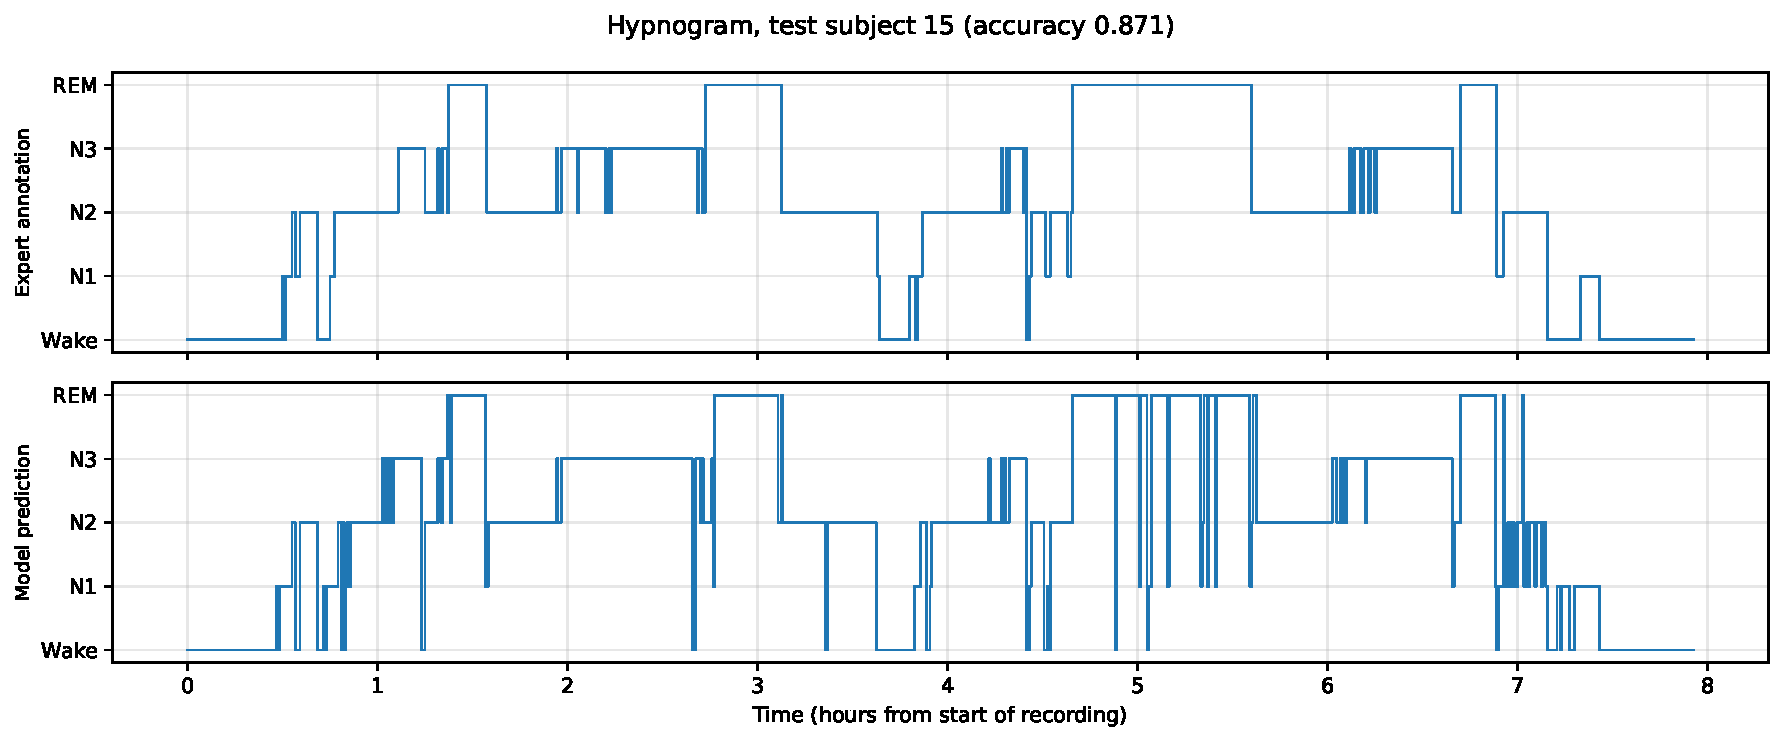
\includegraphics[width=0.88\textwidth]{p2_hypnogram.pdf}
  \caption{Expert annotation and model prediction for test subject~15 (accuracy \num{0.871}).
           The architecture of the night is reproduced; residual errors concentrate at stage
           transitions and in isolated single-epoch flips.}
  \label{fig:hyp}
\end{figure}

%=======================================================================
\section{Changes with respect to the first exam period}
\label{sec:changes}
%=======================================================================

Each row corresponds to one or more \texttt{\# RETAKE CHANGE} comments in the code.

\begin{longtable}{p{4.0cm}p{4.9cm}p{4.5cm}l}
\toprule
\textbf{What} & \textbf{First exam period} & \textbf{Retake} & \textbf{Ref.} \\
\midrule
\endhead
\multicolumn{4}{l}{\textbf{Part I}}\\
\midrule
Wavelet features & 6 sub-band energies; clustering on 2 of them & 173 concatenated \texttt{db4} coefficients, $z$-scored & \S\ref{sec:p1feat} \\
Wiener filter length & $L=256$, assumed & $L=512$, chosen by a sweep & \S\ref{sec:p1L} \\
$S_d$ estimator & Welch on a 140-sample template (averages one segment) & Periodogram of the zero-padded template & \S\ref{sec:p1sd} \\
Extra Butterworth & \SIrange{5}{40}{\hertz} band-pass & Removed; Wiener alone suffices & \S\ref{sec:p1butter} \\
dB convention & $20\log_{10}$ on the PSD plots & $10\log_{10}$ for PSDs, $20\log_{10}$ for $|W|$ & Fig.~\ref{fig:p1wiener} \\
PCA components & 3, from a \SI{90}{\percent} variance rule on 6 dims & 8, from an accuracy sweep on 173 dims & Fig.~\ref{fig:p1pca} \\
Display coefficients & Asserted & Chosen by PC1/PC2 loadings & \S\ref{sec:p1feat} \\
Detector validation & None & Beat count estimated from the label track & Tab.~\ref{tab:p1pct} \\
Reproducibility & Unseeded \texttt{random.randint} & Seeded generator & --- \\
New figures & --- & Raw PSD, $L$ sweep, $S_d$ comparison, PCA sweep, edge effects, subject overlay & --- \\
\midrule
\multicolumn{4}{l}{\textbf{Part II}}\\
\midrule
Band-pass filter & Applied to one epoch only & Applied to every epoch of every subject & \S\ref{sec:p2filt} \\
PSD feature range & 151 bins to \SI{50}{\hertz} & 89 bins, \SIrange{0.5}{30}{\hertz} & \S\ref{sec:p2feat} \\
Band power & Absolute linear power, raw & $\log_{10}$ and relative power & \S\ref{sec:p2feat} \\
Normalisation & Global \texttt{StandardScaler} only & Per-recording $z$-score added & Tab.~\ref{tab:p2prep} \\
EOG/EMG channels & Excluded as features & Five features added & \S\ref{sec:p2emg} \\
EMG rationale & ``EMG is a very slow wave'' & Channel shown to be a \SI{1}{\hertz} envelope; features chosen accordingly & \S\ref{sec:p2emg} \\
Cross-validation & Hand-written loop, 3.5\,h & \texttt{LeaveOneGroupOut} plus \texttt{cross\_validate}, \texttt{n\_jobs=2} & \S\ref{sec:p2cv} \\
Class imbalance & Not addressed & \texttt{class\_weight='balanced'} in the grid & \S\ref{sec:p2cv} \\
Reproducibility & No \texttt{random\_state} on RF/DT & Set on every stochastic estimator & \S\ref{sec:p2cv} \\
ICA fit & All \num{47\,280\,000} samples & Seeded \num{1\,500\,000}-sample subsample, verified & \S\ref{sec:p2ica} \\
Component selection & Not audited & Per-subject table; stable streaming correlation & \S\ref{sec:p2sel} \\
Units & Volts internally, \si{\micro\volt} on axis labels & Converted to \si{\micro\volt} once at load & --- \\
Memory and runtime & \texttt{X} and \texttt{X\_clean\_all} held for all subjects & Streamed per subject; caching & --- \\
New figures & --- & Channel PSD, IC selection, per-class F1, hypnogram, EOG/EMG box plots & --- \\
\bottomrule
\end{longtable}

\paragraph{Summary of the effect.} Part~I: identification accuracy \num{0.558} to
\num{1.000} without dimensionality reduction, and \num{0.773} to \num{0.996} with it.
Part~II: LOSO F1-macro \num{0.678} to \num{0.727}; on the held-out subjects, accuracy
\num{0.744} to \num{0.780} and F1-macro \num{0.610} to \num{0.719}, with every individual
stage improving and N1 rising from F1 \num{0.062} to \num{0.375}.

\end{document}
